% Тут используется класс, установленный на сервере Papeeria. На случай, если
% текст понадобится редактировать где-то в другом месте, рядом лежит файл matmex-diploma-custom.cls
% который в момент своего создания был идентичен классу, установленному на сервере.
% Для того, чтобы им воспользоваться, замените matmex-diploma на matmex-diploma-custom
% Если вы работаете исключительно в Papeeria то мы настоятельно рекомендуем пользоваться
% классом matmex-diploma, поскольку он будет автоматически обновляться по мере внесения корректив
%
\documentclass{matmex-diploma-custom}

\usepackage{amsfonts}
\usepackage{amsmath}
\usepackage{hyperref}
\usepackage{listings}

\lstdefinestyle{customc}{
  belowcaptionskip=1\baselineskip,
  breaklines=true,
  frame=L,
  xleftmargin=\parindent,
  language=C,
  showstringspaces=false,
  basicstyle=\footnotesize\ttfamily,
  keywordstyle=\bfseries\color{green!40!black},
  commentstyle=\itshape\color{purple!40!black},
  identifierstyle=\color{blue},
  stringstyle=\color{orange},
}

\lstset{language=C++, captionpos=b, basicstyle=\footnotesize, breakatwhitespace=true,
breaklines=true, frame=L, style=customc}

\renewcommand{\lstlistingname}{Код программы}



\begin{document}
\filltitle{ru}{
    chair              = {Кафедра Информатики},
    title              = {Анализ возможности и эффективности параллельной реализации алгоритма packJPG},
    type               = {bachelor},
    position           = {студента},
    group              = 461,
    author             = {Шмагринский Игорь Олегович},
    supervisorPosition = {к.\,ф.-м.\,н., доцент},
    supervisor         = {{\sigplace{Н.Ю.~Ловягин}{подпись}}},
    reviewerPosition   = {д.\,ф.-м.\,н., доцент},
    reviewer           = {{\sigplace{T.О. Евдокимова}{подпись}}}
%   university         = {Санкт-Петербургский Государственный Университет},
%   faculty            = {Математико-механический факультет},
%   city               = {Санкт-Петербург},
%   year               = {2013}
}
\filltitle{en}{
    chair              = {Department of Computer Science},
    title              = {Analysis of the possibility and efficiency of the parallel implementation of the packJPG algorithm},
    author             = {Igor Shmagrinsky},
    supervisorPosition = {docent},
    type               = {bachelor},
    supervisor         = {{\sigplace{N.Y.~Lovyagin}{signature}}},
    reviewerPosition   = {docent},
    reviewer           = {{\sigplace{N.N.~Neizvestny}{signature}}}
}
\maketitle
\tableofcontents
\newpage
% У введения нет номера главы
\section*{Введение}

    Быстрое развитие IT технологий позволило в настоящее время даже в мобильных устройствах иметь более чем один процессор, что способствует более быстрому выполнению трудоемких операций при условии использования алгоритмов параллельных вычислений. Однако, еще далеко не все программы и алгоритмы адаптированы для многопроцессорных (многоядерных) архитектур, такие программы работают неэффективно, так как не используют всю мощь современных устройств. Поэтому задача адаптации алгоритмов для параллельных вычислений является важной и актуальной.

 В данной работе расмотрен один из самых эффективных алгоритмов сжатия изображений без потерь PackJPG, который уступает другим алгоритмам этой области лишь по времени работы. Было проведено исследование возможности адаптации данного алгоритма и его реализация для многопроцессорной архитектуры с помощью технологии OpenMP. Выполнена сравнительная оценка времени работы данного алгоритма и его параллельной модификации.

Актуальность работы обусловлена еще и тем, что данный алгоритм дает существенную экономию объема JPEG-изображения (до 26\%) без потери качества, что недоступно при использовании архиваторов, но требует значительных затрат времени на сжатие и распаковку.Скорость кодирования составляет 600 килобайт в секунду. Параллельные вычисления позволили бы сократить это время в несколько раз, доведя до приемлемых величин для небольших изображений. Сложность исследования возможности параллельной реализации алгоритма связана с тем, что спецификация программы и математическое описание недоступно в открытой печати , фактически данная работа выполнялась путем анализа алгоритма по исходному коду.

\section{Предварительные сведения}
Сжатие --- это техника направленная на понижение объемаП

Существует множество разнообразных  техник и стандартов для сжатия мультемедийных данных с потерями.
 Одним из таких стандартов на протяжении многих лет является формат изображений JPEG (ISO/IEC 10918).

\subsection{Стандарт сжатия изображений JPEG}
JPEG---это стандарт сжатия изображений разработаный Joint Photogrphic Experts Group. Он был официально одобрен мировым сообществом в 1992 году.%Пару предложений о стандарте
  Процесс сжатия, осуществляемый алгоритмом, стандарта JPEG состоит из приведенных ниже основных процедур.

\subsubsection{Кодирование}
Хотя \emph{JPEG} файл может быть закодирован разными путями, но самым известным и популярным является \emph{JFIF} кодировние.
Процесс кодирования состоит из нескольких шагов.\\

\textbf{Преобразование цветового пространства} \newline

Основны цвета изображения можно  представить с помощью цветового пространства \emph{RGB}. Такое представление, однако,
%рассказать про RGB и YCrBr
сильно коррелирует, что подразумевает, что это цветовое пространство не очень подходит для независимого кодирования. Так как человеческая зрительная система менее чувствительна к позиции и движению ярких  цветов. Следовательно, целесообразней изпользовать цветовое пространство \emph{YCrBr}.\\

\textbf{Разбиение исходного изображения}\newline

Изображение разбивается на блоки размера  8x8 пикселей, с каждым из которых ведется дальнейшая работа.\\

\textbf{Дискретное косинусное преобразование}\newline

Дальше каждая компонента \emph{(Y,Cr,Br)} каждого блока преобразуется в частотную форма. Для  этого используется двумерное дискретное косинусное преобразование второго типа. Перед вычислением этого преобразования все значения сдвигаются из положительного интервала $[0,255]$в интервал $[---128, 127]$ вычитанием из каждого значения компоненты блока 128. Это действие является обязательным, так как такой интервал значений является одним из требований для дискретного косинусного преобразования. В результате будет получен блок $g_{x,y}$, с которым мы будем работать дальше.\newline

Блок $ g $ преообразуется по следующему принципу:
$$ \ G_{u,v} =
    \frac{1}{4}
    \alpha(u)
    \alpha(v)
    \sum_{x=0}^7
    \sum_{y=0}^7
    g_{x,y}
    \cos \left[\frac{(2x+1)u\pi}{16} \right]
    \cos \left[\frac{(2y+1)v\pi}{16} \right],
  $$
  где:
  \begin{itemize}
  \item{$u$ --- вертикальная пространственная частота для целых чисел $\ 0 \leq u < 8$}
  \item{$v$ --- горизонатальная пространственная частота для целых чисел $\ 0 \leq v < 8$}
  \item{
    $\alpha(u) =
    \begin{cases}
        \frac{1}{\sqrt{2}}, & \mbox{if }u=0 \\1, & \mbox{иначе}
    \end{cases}$
    --- норма, необходимая  для того чтобы преобразование было ортомнормированным.
  }
  \item{
    $\ g_{x,y}$ --- это значение которое содержит в себе пиксель с координатами $\ (x,y)$
  }
    $\ G_{u,v}$ --- это значение которое содержит в себе пиксель с координатами $\ (u,v)$
  }
  \end{itemize}

  После преобразования можно заметить, что значение $ G_{0,0} $  превосходит все остальные, его так же называют
  \emph{коэффициентом DC}. Он определяет основной тон для блока в целом. Его так же можно назвать
  \emph{постоянной компонентой}. Оставшиеся 63 коэффициента (блока 8x8) называют \emph{AC
  коэффициентами}, где AC могут быть установлены для запасных комп                                                  онент.
  Преимущество дискретного косинусного преобразования --- возможность вычислить основной оттенок блока (сигнала).\\

\textbf{Квантование}\newline

Человеческий глаз  хорошо приспособлен замечать маленькие различия в яркости на относительно больших расстояниях, но плохо отличает точную силу яркости на высоких частотах. Это позволяет значительно уменьшить количество информации о высокого частотных компонентах. Данную операцию можно  осуществить простым делением значения  каждой компоненты в частотном диапозоне на константу и последующим округлением этого значения ближайшим целым числом. Это действие, единственное во всем процессе сжатия при котором происходит потеря данных, в отличии от дискретного косинусного пребразования, которое выполняет вычисления с выской точностью. Как результат, многие компоненты оказваются равны  нулю или их значение очень близко к нулю, как следствие они занимают меньше бит в памяти.

%The human eye is good at seeing small differences in brightness over a relatively large area, but not so good at distinguishing the exact strength of a high frequency brightness variation. This allows one to greatly reduce the amount of information in the high frequency components. This is done by simply dividing each component in the frequency domain by a constant for that component, and then rounding to the nearest integer. This rounding operation is the only lossy operation in the whole process (other than chroma subsampling) if the DCT computation is performed with sufficiently high precision. As a result of this, it is typically the case that many of the higher frequency components are rounded to zero, and many of the rest become small positive or negative numbers, which take many fewer bits to represent.
Подобные процессы, когда процедура построения чего-либо ведeтся с помощью набора дискретных (в нашем случае целых) величин, называется \emph{квантованием}.

Элементы \emph{матрицы квантования} управляют коэфициентом сжатия. Чем больше значение компонент, тем больше будет потеря изображения в качетсве. Типичная матрица квантования (качество ухудшается примерено на 50\%, утверждена как часть стандарта JPEG), выглядит следующим образом:
%The elements in the quantization matrix control the compression ratio, with larger values producing greater compression. A typical quantization matrix (for a quality of 50% as specified in the original JPEG Standard), is as follows:
$$ Q=
     \begin{bmatrix}
      16 & 11 & 10 & 16 & 24 & 40 & 51 & 61 \\
      12 & 12 & 14 & 19 & 26 & 58 & 60 & 55 \\
      14 & 13 & 16 & 24 & 40 & 57 & 69 & 56 \\
      14 & 17 & 22 & 29 & 51 & 87 & 80 & 62 \\
      18 & 22 & 37 & 56 & 68 & 109 & 103 & 77 \\
      24 & 35 & 55 & 64 & 81 & 104 & 113 & 92 \\
      49 & 64 & 78 & 87 & 103 & 121 & 120 & 101 \\
      72 & 92 & 95 & 98 & 112 & 100 & 103 & 99
     \end{bmatrix}.
$$

Квантование коэффициентов матрицы  G, полученной на предыдущем шаге, происходит следующим образом:
% The quantized DCT coefficients are computed with
е
$$B_{j,k} = \mathrm{round} \left( \frac{G_{j,k}}{Q_{j,k}} \right) \mbox{ для } j=0,1,2,\ldots,7; k=0,1,2,\ldots,7$$

 % B_{j,k} = \mathrm{round} \left( \frac{G_{j,k}}{Q_{j,k}} \right) \mbox{ for } j=0,1,2,\ldots,7; k=0,1,2,\ldots,7

  %where G is the unquantized DCT coefficients; Q is the quantization matrix above; and B is the quantized DCT coefficients.
  Полученная матрица B, отправляется на следующий шаг, где будет произвоидиться ее энтропийное кодирование.\\
  %Using this quantization matrix with the DCT coefficient matrix from above results in:

\textbf{Энтропийное кодирование}\\

\emph{Энтропийное кодирование} — кодирование последовательности значений с возможностью однозначного восстановления с целью уменьшения объёма данных (длины последовательности) с помощью усреднения вероятностей появления элементов в закодированной последовательности.

 В JPEG формате реализация включает в себя переопределение порядка компонент изображения в виде \emph{"зиг-зага"} (рис. 1) и дальнейшее сжатие методом \emph{кодирования повторов}, который группирует похожие повторяющие значения вместе. Затем к получивишейся последовательности применяется \emph{Код Хаффмана}.\\
    \begin{figure}
      \centering
        \reflectbox{%
          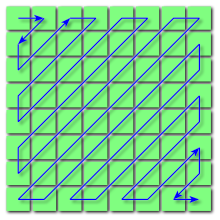
\includegraphics[width=0.5\textwidth]{images/zig-zag.png}}
      \caption{Порядок "зиг-заг" в котором кодируются компонеты блока.}
    \end{figure}
 %Entropy coding is a special form of lossless data compression. It involves arranging the image components in a "zigzag" order employing run-length encoding (RLE) algorithm that groups similar frequencies together, inserting length coding zeros, and then using Huffman coding on what is left.

 %  The previous quantized DC coefficient is used to predict the current quantized DC coefficient. The difference between the two is encoded rather than the actual value. The encoding of the 63 quantized AC coefficients does not use such prediction differencing.

Для описания процесса сжатия  данных представленных в "зиг-заг" порядке - кодирования повторов, введем некоторые определения:

 %The process of encoding the zig-zag quantized data begins with a run-length encoding explained below, where:

\begin{itemize}
    \item{
        $x$ --- ненулевой AC коэфициент, получившийся после квантования;
    }
    %x is the non-zero, quantized AC coefficient.
    \item{
        $RUNLENGTH$ --- число нулей перед ненулевым AC коэффициентом;
        %???
    }
     %RUNLENGTH is the number of zeroes that came before this non-zero AC coefficient.
     \item{
        $SIZE$ --- число бит, требуемых чтобы представить $x$;
     }
      %SIZE is the number of bits required to represent x.
    \item{
        $AMPLITUDE$ --- побитовое представление $x$.
    }
     %AMPLITUDE is the bit-representation of x.
\end{itemize}

Кодирование повторов работает исследуя каждый  ненулевой AC коэффицинт $x$ и определяя, как много нулей следует перед ним. C этой иноформацией создаются два \emph{символа}:

 %The run-length encoding works by examining each non-zero AC coefficient x and determining how many zeroes came before the previous AC coefficient. With this information, two symbols are created:

  $$ \begin{bmatrix}
        Symbol 1 & Symbol 2 \\
        RUNLENGTH, SIZE& AMPLITUDE\\

       \end{bmatrix}. $$\\

  Оба числа RUNLENGTH и SIZE  хранятся в одном и том же байте, под каждый из них отводится по 4 бита. Так значения любого из них не превосходит 64.

 %Both RUNLENGTH and SIZE rest on the same byte, meaning that each only contains four bits of information. The higher bits deal with the number of zeroes, while the lower bits denote the number of bits necessary to encode the value of x.

Так же в стандарт JPEG определены специальные символы, которые означают окочание блока (\emph{EOB}), и еще один на случай? когда встречаются более более 15 нулей подряд, до достижения ненулевого коэффицинта, тогда символ кодируется специально как: (15, 0) (0).
 %This has the immediate implication of Symbol 1 being only able store information regarding the first 15 zeroes preceding the non-zero AC coefficient. However, JPEG defines two special Huffman code words. One is for ending the sequence prematurely when the remaining coefficients are zero (called "End-of-Block" or "EOB"), and another when the run of zeroes goes beyond 15 before reaching a non-zero AC coefficient. In such a case where 16 zeroes are encountered before a given non-zero AC coefficient, Symbol 1 is encoded "specially" as: (15, 0)(0).

 Весь процесс продолжается до тех пор? пока не будет достигнут символ окончания блока. Определенный как символ  EOB --- (0,0).\\

 %The overall process continues until "EOB" – denoted by (0, 0) – is reached.

 %With this in mind, the sequence from earlier becomes:

\subsubsection{Декодирование}

Декодирование для отображения изображения состоит из тех же шагов, выполняемых в обратном порядке.

%Decoding to display the image consists of doing all the above in reverse.

Возьмем раскодированую матрицу коэффициентов, полученную после примения к ней дешифрования кода Хаффмана и декодирование повторов. И расположим символы этой последовательности в правильном порядке. В результате получится матрица $B$, являющуюся результатом шага квантования.
%Taking the DCT coefficient matrix (after adding the difference of the DC coefficient back in)
Затем умножим матрицу $B$ на матрицу квантования $Q$ по Адамару. В результате получим матрицу $F$

%and taking the entry-for-entry product with the quantization matrix from above results in
$$ F = B \circ Q,$$

которая очень похожа на оригинальную  матрицу $G$, явяляющуюся результатом дискретного косинусного преобразования.

%which closely resembles the original DCT coefficient matrix for the top-left portion.

Следующим шагом является применение обратного косинусного преобразования, которое можно описать следюущим образом:

%The next step is to take the two-dimensional inverse DCT (a 2D type-III DCT), which is given by:

$$f_{x,y} =
 \frac{1}{4}
 \sum_{u=0}^7
 \sum_{v=0}^7
 \alpha(u) \alpha(v) F_{u,v}
 \cos \left[\frac{(2x+1)u\pi}{16} \right]
 \cos \left[\frac{(2y+1)v\pi}{16} \right]
,
$$
%where

где

\begin{itemize}
\item{
$\ x$ столбец пикселей $\ 0 \leq x < 8$;
}
\item{
$\ y$ строка пикселей $\ 0 \leq y < 8$;
}
\item{
$\ F_{u,v}$ это компонента матрицы коэффициентов полученая на предыдущем шаге с координатам $\ (u,v)$;
}
\item{
$\ f_{x,y}$ --- значение полученой компоненты с координатами $\ (x,y)$.
}
\end{itemize}

Затем значение каждой компоненты округляются до ближайшего целого числа, так как изначально значение компоненты целочисленное, и к каждому значению прибавляется 128. На этом процедура декодирования заканчивается. И мы получаем изображениe практически идентичное оригиналу.
%Rounding the output to integer values (since the original had integer values) results in an image with values (still shifted down by 128)



%Notice the slight differences between the original (top) and decompressed image (bottom), which is most readily seen in the bottom-left corner.

%and adding 128 to each entry

%This is the decompressed subimage. In general, the decompression process may produce values outside the original input range of [0, 255]. If this occurs, the decoder needs to clip the output values keep them within that range to prevent overflow when storing the decompressed image with the original bit depth.

%The decompressed subimage can be compared to the original subimage (also see images to the right) by taking the difference (original − uncompressed) results in the following error values:


%with an average absolute error of about 5 values per pixels (i.e., \frac{1}{64} \sum_{x=0}^7 \sum_{y=0}^7 |e(x,y)| = 4.9197).

%The error is most noticeable in the bottom-left corner where the bottom-left pixel becomes darker than the pixel to its immediate right.

\subsection{Сжатие JPEG изображений без потерь}
Как мы могли заметить, в основе оригинального алгоритма JPEG лежит сжатие по коду Хаффмена. Как известно, за последнее время появилось множество других алгоритмов энтропийного кодирования, которые гораздо эффективнее компрессируют информацию в сравнении с данным алгоритмом. Это повлекло за собой образование целого класса алгоритмов, которые позволяют нам дальнейшее сжатие JPEG изображений без  потери в качестве.

    Одним из представителей этого класса алгоритмов является программа packJPG, в основе которой лежит алгоритм с одноименным названием. Преимуществом данного алгоритма является высокая степень сжатия,а недостатком  --- низкая скорость кодирования, в сравнение с алгоритмами подобного рода.

    До недавнего времени код алгоритма был закрыт, но в 2014 году был опубликован и получил лицензию GPL3, что позволило в данной работе проанализировать его исходный код, понять основные идеи алгоритма и его реализации.


\subsection{Технология OpenMP}
В ходе данной работы  проведена попытка адаптировать исходный алгоритм packJPG для многопроцессорных архитектур и создать его более эффективную реализацию. Код исходного проекта написан на языке С++ и поэтому для реализации была выбрана технология OpenMP, которая зарекомендовала себя как простой и удобный инструмент для многопоточного программирования.
    Важным достоинством технологии OpenMP является возможность реализации так называемого инкрементального программирования, когда программист постепенно находит участки в программе, содержащие ресурс параллелизма, с помощью предоставляемых механизмов делает их параллельными, а затем переходит к анализу следующих участков. Таким образом, в программе нераспараллеленная часть постепенно становится всё меньше. Такой подход значительно облегчает процесс адаптации последовательных программ к параллельным компьютерам, а также отладку и оптимизацию.

\section{Алгоритм packJPG}

PackJPG --- это пограмма специально разработанная для дальнейшего сжатия JPEG изображений без потерь. Обычно ей удается уменьшить размер файла JPEG изображения  примерно на 20\%.
% packJPG is a compression program specially designed for further compression of JPEG images without causing any further loss. Typically it reduces the file size of a JPEG file by 20%.

В данном подходе JPEG файл первоначально декодируется в коэффициенты, получившиеся после шага квантования.
Далее эти коэффициенты перегруппируются в 64 изображения для каждой цветовой компоненты, содержащейся в исходном изображении. Каждое сгруппированное изображение содержит все коэффициенты 'подзоны' в соответствии с  двумерной  базисной функции дискретного косинусного преобразования(DCT коэффициенты).

Обычно существуют статистические зависимости между соответсвующими DCT коэффициентами соседних блоков --- в стандартном алгоритме JPEG эта избыточность, в некотором роде, подавляется только лишь дифференциальным кодированием коэффициентов 'подзоны'.

Особенностью данного подхода являются следующие шаги, которые применяются к раскодированным коэффициентам:
Paeth предиктор, использование списков концов блоков, оптимизированное сканирование и арифметическое кодирование, как один из вариантов энтропийного кодирования. Рассмотрим каждый их них более детально.

\subsection{Paeth предиктор}

Раскодированные и сгруппированные коэффициенты представляют собой уменьшенную копию исходного изображения. Следовательно,к ним  можно применить те же техники декорреляции, что используются для изображений в градации серого.
Одной из самых простых и эффективных подоюных техник явяется Paeth предиктор, который описан в спецификации формата PNG. Его предназначение в следующем: он пытается выбрать лучшее возможное направление для каждого пикселя. Вычисляется простая линейная функция из трех соседних пикселей (левый, верхний, левый-верхний), выбирается тот пиксель, который ближе всего к результату.

\subsection{Использование списков концов блоков}
В макроблоке из 64 коэффициентов, отсортированных в зиг-заг порядке, \emph{конец блока} определяется, как позиция после последнего ненулевого коэффициента. Все концы блоков каждого макроблока из одной цветовой компоненты группируются вместе в форме списка концов блоков для этой цветовой компоненты.

В стандартном алгоритме сжатия JPEG большинство коэффициентов после шага квантования принимают нулевые значения и на самом деле большая часть из них встречается в конце зиг-заг упорядоченных коэффициентов. Следовательно, концы блоков могут быть использованы для эффективной группировки и кодирования последних нулей. Такой же подход применятся в стандартном алгоритме JPEG, где не используются списки концов блоков. Там концы блоков кодируются с помощью специального символа.

В подходе packJPG вышеуказанные списки используются для дополнительной цели. Можно предположить, что чем позже появляется конец блока, то тем больше высокочастотных компонент содержится в макроблоке.

В данном подходе блоки 8x8 группируются в соответсвии со значениями концов блоков. Каждая группа блоков кодируется независимо от других групп. Оптимальное количество уровней варьируется от изображения к изображению. Это зависит от размера изображения. Границы уровней вычисляются через линейные квантили списка концов блоков.

\subsection{Оптимизированное сканирование}
Коэффициенты кодируются для "подзоны", коэффициент за коэффициентом, используя статистическую модель первого порядка. Но в отличии от стандартного алгоритма в packJPG обход компонент блока делается не в прямом порядке, а в специальном.

Так например, обычный горизонтальный обход применяется только для компонент лежащих ниже диагонали блока. Компоненты лежащие выше диагонали кодируются с помощью вертикального обхода. А все элементы диагонали блока кроме DC коэффициента кодируются в порядке основанном на на нескольких кривых Гильберта.

\subsection{Арифметическое кодирование}

В данном подходе используются статистические модели разных порядков для кодирования разных типов данных с помощью алгоритма  \emph{арифметического кодирования}.

Так например, JPEG заголовок, который необходим для сжатия без потерь, будет использовать статистическую модель первого порядка.

Cписки конца блоков будут компрессироваться с помощью двуразмерной статистичкской модели. Для каждого значения конца блока в качесве контекста статистической модели используются значения верхнего и левого блоков.

Коэффициенты, получившиеся после дискретного косинусного преобразования, кодируются в соответсвии со знаком значения, его абсолютной величиной и категорией. Эту схему можно объснить следующим образом.

В большинстве случаев знак коэффициентов не может быть сжат ниже чем до 1 бита на коэффициент. Используя статистическую модель первого порядка и оптимизированный порядок обхода компонент, описанный выше, их сжатый размер не будет превышать одного бита на знак.

Оставшиеся абсолютные значения коэффициентов дискретного косинусного преобразования кодируются с помощью схемы очень похожей на ту, что  приведена в стандарте JPEG под  названием \emph{Variable Length Integer}. Cначала значения разбиваются по категориям, после обхода сгруппированных коэффициентов с помощью оптимизрованного порядка, мы будем применять для кодирования последовательности статистическую модель первого порядка, используя предшествующие значения как контекст для модели.

Полученные коэффициенты отправляются на еще один этап сжатия, где будут сжиматься опять таки с помощью статистической модели первого порядка, но в качетсве контекста уже будет использоваться категория. Значения категорий были вычислены империческим путем.

\section{Анализ возможности реализации с помощью технологии OpenMP}
Анализ возможности  реализации включает в себя следующие этапы: анализ существующего кода приложения \emph{packJPG}, рефакторинг существующего кода, поиск узких мест алгоритма, модификация с помощью технологии OpenMP, оценка эффиктивности осуществленной модификации. Рассмотрим каждый из них более подробно.

\subsection{Анализ существующего кода приложения}
Исходный код приложения состоит более чем из 10000 строк, и этот достаточно внушительный объем кода содержится в 5 файлах. Поэтому значительная часть времени была затрачена на изучнение структуры приложения и анализ деталей реализации алгоритма \emph{packJPG}.

Основной код приложения расположен в файле \emph{packjpg.cpp}. PackJPG является полноценным программным обеспечением для сжатия JPEG изображений, и большая часть исходного кода предназначена для предоставления удобного контроля за функционалом программы. Так для \emph{Windows} и \emph{MacOS} написана реализация графического пользовательского интерфейса, а также для всех платформ реализован \emph{интерфейс командной строки}.

  Эта часть программа, имеет малую вычислетельную сложность и не относится к алгоритмам компрессии. Поэтому будут рассмотрены компоненты кода, которые ответсвенны за сам процесс сжатия.

\subsubsection{JPEG кодирование и декодирование}
Весь код, ответственный за кодировние  и декодирование сжатия формата JPEG, содержится в двух основных методах. Так процедурой по извлечению всей структуры JPEG изображения, представленной в главе 1, занимается метод \emph{ decode\_jpeg }, а за обратную процедуру отвечает метод \emph{ recode\_jpeg }.

%Кусок кода ответсвенный за кодирование и декодирование и описание того, что он делает
\subsubsection{Предиктивное кодирование}
Данная релизация поддерживает несколько вариантов линейного предиктивного кодирования, описанного в п. 2.1. Присутствует возможность опционально выбирать тип предиктивного кодирования для лучшего сжатия.
    Первая реализация --- это \emph{loco-i} предиктор и ответсвенный за него метод: \emph{int plocoi( int a, int b, int c )}, второй --- \emph{dc\_coll\_predictor}, предиктор, используемый для массива данных и реализующий его метод: \emph{int dc\_coll\_predictor( int cmp, int dpos )}. Третья реализация --- предиктор, используемый для DC коэффициентов, базирующийся на дискретном косинусном преобразовании: \emph{int dc\_1ddct\_predictor( int cmp, int dpos )}
%Кусок кода ответсвенный за предиктовное кодирование
\subsubsection{Арфимитическое кодирование}
Основным компонентом определяющим интерфейс и являющимся кодировщиком и декодировщиком последовательности \emph{символов} является класс \emph{aricoder} со следующими публичными методами, представленными на листинге:


\begin{lstlisting}
class aricoder {
public:
    aricoder(iostream *stream, int iomode);

    ~aricoder(void);

    void encode(symbol *s);

    unsigned int decode_count(symbol *s);

    void decode(symbol *s);
    ...
\end{lstlisting}

Под \emph{символом} понимают следующую структуру, которая хранит информацию о вероятностном диапозоне кодируемого числа и его частоте, код структуры приведен в следующем листинге:

\begin{lstlisting}
struct symbol {
    unsigned int low_count;
    unsigned int high_count;
    unsigned int scale;
};
\end{lstlisting}

Основным классом, который используется для энтропийного кодирования, в случае арифметического кодирования, является статистическая модель. В данном коде существует две модификации: \emph{model\_s} --- модель первого порядка и \emph{model\_b} --- двумерная модель. Они имеют схожий интерфейс. Например класс \emph{model\_s} имеет следующую структуру:

\begin{lstlisting}
class model_s {
public:

    model_s(int max_s, int max_c, int max_o, int c_lim);

    ~model_s(void);

    void update_model(int symbol);

    void shift_context(int c);

    void flush_model(int scale_factor);

    void exclude_symbols(char rule, int c);

    int convert_int_to_symbol(int c, symbol *s);

    void get_symbol_scale(symbol *s);

    int convert_symbol_to_int(int count, symbol *s);

    bool error;


private:

    // unsigned short* totals;
    unsigned int *totals;
    char *scoreboard;
    int sb0_count;
    table_s **contexts;
    table_s **storage;

    int max_symbol;
    int max_context;
    int current_order;
    int max_order;
    int max_count;
\end{lstlisting}

Для хранения контекста моделей используются специальные таблицы --- это структуры данных, содержащие следующую информацию: счетчики для каждого символа, содержащегося в таблице; ссылки на таблицы порядком выше и ниже; накопительные счетчики. Листинг cтруктуры \emph{table}, используемой в \emph{model\_b}, будет привиден ниже. Похожая реализация имеется и для класса \emph{model\_s} и описана в структуре под названием \emph{table\_s}:

\begin{lstlisting}
struct table {
    // counts for each symbol contained in the table
    unsigned short *counts;
    // links to higher order contexts
    struct table **links;
    // link to lower order context
    struct table *lesser;
    // accumulated counts
    unsigned int scale;
};
\end{lstlisting}
\subsection{Рефакторинг существующего кода}
Как говорилось в предудущей главе, код проекта плохо поддавался анализу и требовал большого времени для поиска, той или иной компоненты. Еще одной особенностью кода данного приложения являлется его процедурный стиль. К основным недостаткам также можно отнести длинные методы, многократное дублирование кода, расходящиеся модификации.

Очевидно, что данный код требовал рефакторнинга, который был произведен. Основные проблемы и частные случаи их  решения будут рассмотрены в следующих пунктах.

\subsubsection{Реструктуризация исходного кода}
Первым этапом в  подготовке кода к дальнейшей разработке стала декомпозиция больших файлов и выделение оттуда компонент с определенной зоной ответственности. Компоненты  были разбиты на группы по области применения и распределенны по соответствующим пакетам. Например, такие классы как \emph{model\_s}, \emph{model\_b} и др. оказались в пакете \emph{aricoder}, ответсвенном за арифмитичское кодирование.

Так же были выделены и сформированы пакеты \emph{gui} и \emph{utils}, отвечающие за графический пользовательский интерфейс и различные утилитные классы.

Первоначальная сборка проекта осуществлялась с помощью обычного \emph{Makefile}, что осложняло ее рутинными процедурами и не позволяло гибко управлять ею. Одной из задач была интеграция библиотки OpenMP в данное приложение, но стало бы мешать другим разработчикам, у которых непредустановлена эта библиотека в системе,вынуждая  заниматься ее инсталяцией. Поэтому для сборки был выбран такой нструмент как \emph{СMake}, для которого уже реализован модуль \emph{FindOpenMP}. Он отвечает за поиск библиотеки OpenMP, а в случае, если она не обнаружена --- директивы данной библиотеки игнорируются.

\subsubsection{Дублирование кода}
Дублирование кода --- это случай, когда два фрагмента кода выглядят почти одинаково. В данном исходном коде такого рода дублирования достаточно много. Это понижает читабельность кода и делает его структуру более сложной, ветвистой и непонятной.

Например, код процедуры сортировки массива встречается в нескольких  местах и представляет собой обычную \emph{сортировку вставками}. Для избавления от дублирования в данном случае было использовано извлечение метода или  просто перенос процедуры сортировки в один из утилитных  классов. Так в класс \emph{common\_utils} был извлечен метод \emph{insertion\_sort}, который можно увидеть в листинге приведенном ниже:

\begin{lstlisting}
class common_utils
{
    ...
    template <class T>
    static void insertion_sort(T* values, int size )
    {
        bool done;
        T swap;
        int i;

        // sort data first
        done = false;
        while ( !done ) {
           ...
        }

    }
    ...
}
\end{lstlisting}

\subsubsection{Длинные методы}
Еще одной особенностью данного исходного кода является высокая цикломатическая сложность некоторых методов и длина их кода. Так например, методы \emph{decode\_jpeg} или \emph{encode\_jpeg} имеют длину более 300 строк. Это не является целeсообразным, и делает такой код очень трудночитаемым и плохо переиспользуемым. Такие участки кода необходимо декомпозировать. Для разрешения этой проблемы была проведена декомпозиция кода, извлечены методы с определенными обязанностями, переменные были  заменены вызовами методов.

\subsection{Модификация с помощью технологии OpenMP}

\subsubsection{Поиск узких мест программы}
В предыдущих пунктах этой главы было замечено, что программа имеет большое количество процедур и кода, следовательно первым делом возникла идея парллельной реализации тех методов, которые исполняются чаще всего. Таким образом, распараллеливание этих методов могло дать максимальный выигрыш в производительности.

Для оценки времени исполнения кода каждого метода использовался профайлер \emph{valgrind}, который имеет бесплатную лицензию, гибкую настройку и обладает всем требуемым функционалом. На основе результатов профайлера было установлено, что самой долгой по времени выполнения является шаг арифмитеческого кодирования последовательности элементов. Дольше всего алгоритм находится в методах \emph{shift\_context} и \emph{update\_model} классов статистических моделей \emph{model\_s} и \emph{model\_b}.

\subsubsection{Параллельные модификации}
Была произведена параллельная реализация нескольких десятков участков кода.Рассмотрим несколько примеров таких модификаций более подробно.
При первоначальной оценке данного алгоритма предполагалось, что удастся добиться высокого уровня распараллеливания за счет блочных  структур, которые активно задействованы в формате JPEG. Следовательно в исходном коде часто используется такая конструкция как цикл, что являлется благоприятным условием для многопоточного программирования.

Одним из самых популярных видов распараллеливания стало распараллеливание существующих циклов \emph{for}. Так например неэффективная \emph{сортирвка вставками}:

 \begin{lstlisting}
 template <class T>
     static void insertion_sort(T* values, int size )
     {
         bool done;
         T swap;
         int i;
         done = false;
         while ( !done ) {
             done = true;
             for ( i = 1; i < size; i++ )
                 if ( values[ i ] < values[ i - 1 ] ) {
                     swap = values[ i ];
                     values[ i ] = values[ i - 1 ];
                     values[ i - 1 ] = swap;
                     done = false;
                 }
         }

     }
 \end{lstlisting}

 была заменена параллельной реализацией быстрой сортировки, что дало прирост примерно в 2\%. Фрагмент данной модификация отражен на следующем листинге:

 \begin{lstlisting}
 template<class T>
     static void sort(T *a, int n) {
         long i = 0, j = n;
         float pivot = a[n / 2];
         do {
             while (a[i] < pivot) i++;
             while (a[j] > pivot) j--;
             if (i <= j) {
                 std::swap(a[i], a[j]);
                 i++;
                 j--;
             }
         } while (i <= j);
         if (n < 100) {
             if (j > 0) sort(a, j);
             if (n > i) sort(a + i, n - i);
             return;
         }
         #pragma omp task shared(a)
         if (j > 0) sort(a, j);
         #pragma omp task shared(a)
         if (n > i) sort(a + i, n - i);
         #pragma omp taskwait
     }

 };
 \end{lstlisting}

Так как одним из этапов алгоритма является выполнение дискретного косинусного преобразования и обратного дискретного косинусного преобразования. Многие процедуры связаны с транформацией блоков или же с их  обходом, поэтому эти участки содержат элементарные циклы которые хорошо поддаются распараллеливанию. Примером может служить метод используемый на этапе обратного косинусного преобразования \emph{int idct\_2d\_fst\_8x8( signed short* F, int ix, int iy )}:

 \begin{lstlisting}
 inline int idct_2d_fst_8x8( signed short* F, int ix, int iy )
 {
 	int idct;
 	int ixy;
 	int i;

 	ixy = ( ( iy * 8 ) + ix ) * 64;

 	idct = 0;
 	for ( i = 0; i < 64; i++ )
 		idct += F[ i ] * icos_idct_8x8[ ixy++ ];

 	return idct;
 }
 \end{lstlisting}

И после паралельной модификации используя параллелизм циклов и опцию редукции библиотеки openMP, была получена следующая модификация.

\begin{lstlisting}
int idct_2d_fst_8x8( signed short* F, int ix, int iy )
{
	int idct;
	int ixy;
	int i;
	ixy = ( ( iy * 8 ) + ix ) * 64;
	idct = 0;
    #pragma omp parallel for reduction(+:idct)
	for ( i = 0; i < 64; i++ )
		idct += F[ i ] * icos_idct_8x8[ixy + i];
	return idct;
}
\end{lstlisting}

\subsubsection{Проблемы модфикации}
Основной проблемой, которая были обнаружена во время реализации --- это то, что самым трудоемким участком кода являются методы связанные с обновлением и обработкой статистической модели. Ярким примером является метод \emph{shift\_context}, приведенный в данном листинге.

\begin{lstlisting}
void model_s::shift_context( int c )
{
    table_s* context;
    int i;

    // shifting is not possible if max_order is below 1
    // or context index is negative
    if ( ( max_order < 1 ) || ( c < 0 ) ) return;

    // shift each orders' context
    for ( i = max_order; i > 0; i-- ) {
        // this is the new current order context
        context = contexts[ i - 1 ]->links[ c ];

        // check if context exists, build if needed
        if ( context == NULL ) {
            // reserve memory for next table_s
            context = ( table_s* ) calloc( 1, sizeof( table_s ) );
            if ( context == NULL ) ERROR_EXIT;
            // set counts NULL
            context->counts = NULL;
            // setup internal counts
            context->max_count  = 0;
            context->max_symbol = 0;
            // link lesser context later if not existing, this is done below
            context->lesser = contexts[ i - 2 ]->links[ c ];
            // finished here if this is a max order context
            if ( i == max_order )
                context->links = NULL;
            else {
                // build links to higher order tables otherwise
                context->links = ( table_s** ) calloc( max_context, sizeof( table_s* ) );
                if ( context->links == NULL ) ERROR_EXIT;
                // add lesser link for higher context (see above)
                contexts[ i + 1 ]->lesser = context;
            }
            // put context to its right place
            contexts[ i - 1 ]->links[ c ] = context;
        }

        // switch context
        contexts[ i ] = context;
    }
}
\end{lstlisting}

Как можно увидеть, этот метод требует строго последовательного выполнения, то есть код выполняется связно, и следующий результат зависит от предыдущего. Такие участки кода практически не поддаются распараллеливанию, и единственным вариантом стало введение параллельных секций внутри тела цикла, которые работают с независимыми участками кода:

\begin{lstlisting}
#pragma omp parallel {
    context->max_count  = 0;
    context->max_symbol = 0;
    // link lesser context later if not existing, this is done below
    context->lesser = contexts[ i - 2 ]->links[ c ];
    // finished here if this is a max order context
    if ( i == max_order )
        context->links = NULL;
    else {
        // build links to higher order tables otherwise
        context->links = ( table_s** ) calloc( max_context, sizeof( table_s* ) );
        if ( context->links == NULL ) ERROR_EXIT;
        // add lesser link for higher context (see above)
        contexts[ i + 1 ]->lesser = context;
    }
}
\end{lstlisting}

Однако, после проведения тестов выяснилось, что такая модификация не приносит положительного эффекта. И данный метод пришлось оставить без модификаций.

%Объяснеие почему не получилось распараллпелить некоторые участки кода с примером.
\section{Результаты}
Для оценки внесенных модификаций, были проведены тесты производительности. Тесты  проводились на компьютере c процессором Intel Celeron 1007U, имеющим два физических и два вирутальных ядра с частотами 1.5 GHz. Сравнительная таблица результов работы до и после модификации представлена ниже:


\begin{center}
    \begin{tabular}{ | p{5cm} | p{5cm} | p{5cm}|}
    \hline
    Размер изображения (пикс./мегабайт) & Исходная реализация (сек.) & Параллельная модификация (сек.) \\ \hline
    400x400/0.0136 & 0.027 & 0.021 \\ \hline
    1920x1080/1.075 & 1.387 & 1.317 \\ \hline
    4000x4000/3.500 & 5.22 & 5.01 \\
    \hline
    \end{tabular}
\end{center}


В среднем был получен прирост в производительности приблизительно на 3-4\%, что является приемлимым, но не оптимальным результатом. Данный результат связан прежде всего с высокой связностью алгоритма packJPG, где многие итеративные элементы кода не поддаются полному распараллеливанию.

\section*{Заключение}
В настояещей дипломной работе был проведен анализ возможности и эффективности параллельной реализации на примере алгоритма packJPG, являющегося компонентом одноименной программы.
% защита основных положений, отличающих это дипломное исследование от работ предшественников;
В процессе выполнения работы был изучен стандарт изображений JPEG и его представлениe, кодированиe и декодированиe. Также осуществлен анализ алгоритмов сжатия JPEG без потерь и выявлены основые преимущества и недостатки алгоритма packJPG.


В ходе основного этапа работы был осуществлен анализ кода и выявлены  его основноые компоненты. Данная процедура потребовала массивного рефакторинга существующего кода. На основе этого было выполнено более детальное описание алгоритма.

Параллельная  реализация осуществлялась с помощью техники инкременатального программирования. Процедура реализации выполнялась итеративно.Итерация представляла из себя параллельную реализацию фрагмента кода и оценку эффектвиности этой модификации. В некоторых частях кода ее произвести оказалось невозмоожным, в связи со спецификой программы.

Проведенная работа может быть продолжена в виде реализации данного алгоритма для графических вычислительных устройств, так как код наполенен большим количеством циклов, работающих с одноразмерными и двуразмерными векторами. Видеокарта имеет болшое количеством ядер для вычисления, что должно увеличить эффективность проведеной реализации, если ее удастся адапировать для видеокарт.

\nocite{*}
\bibliographystyle{ugost2008}
\bibliography{diploma}
\end{document}